% THIS IS A LATEX TEMPLATE FILE FOR PAPERS INCLUDED IN THE
% *Anthology of Computers and the Humanities*. ADD THE OPTION
% 'final' WHEN CREATING THE FINAL VERSION OF THE PAPER. 
% DO NOT change the documentclass
%\documentclass[final]{anthology-ch} % for the final version
\documentclass{anthology-ch}         % for the submission

% LOAD LaTeX PACKAGES
\usepackage{booktabs}
\usepackage{graphicx}
% ADD your own packages using \usepackage{}

% TITLE OF THE SUBMISSION
% Change this to the name of your submission
\title{Unstable data, Unanticipated uses}

% AUTHOR AND AFFILIATION INFORMATION
% For each author, include a new call to the \author command, with
% the numbers in brackets indicating the associated affiliations 
% (next section) and ORCID-ID for each author.  
\author[1]{Rebecca Sutton Koeser}[
  orcid=0000-0002-8762-8057
]

\author[1]{Mary Naydan}[
  orcid=0000-0002-7960-3175
]

% While we encourage including ORCID-IDs for all authors, you can
% include authors that do not have one by definining an empty ID.
%\author[1,2]{Meredith Martin}[
\author[1,2]{Meredith Martin}[
  orcid=0000-0003-0214-8757
]

% There should be one call to \affiliation for each affiliation of
% the authors. Multiple affiliations can be given to each author
% and an affiliation can be given to multiple authors. 
\affiliation{1}{Center for Digital Humanities, Princeton University, Princeton, New Jersey, USA}
% \affiliation{2}{Another Department, Another University, Another City, Another Country}

% KEYWORDS
% Provide one or more keywords or key phrases seperated by commas
% using the following command
\keywords{humanities data, unstable data, reproducibility}

% METADATA FOR THE PUBLICATION
% This will be filled in when the document is published; the values can
% be kept as their defaults when the file is submitted
\pubyear{2025}
\pubvolume{1}
\pagestart{1}
\pageend{1}
\conferencename{Proceedings of Conference XXX}
\conferenceeditors{Editor1 Editor2}
\doi{00000/00000}  

\addbibresource{bibliography.bib}

%%%%%%%%%%%%%%%%%%%%%%%%%%%%%%%%%%%%%%%%%%%%%%%%%%%%%%%%%%%%%%%%%%%%%%%%%%%
% HERE IS THE START OF THE TEXT
\begin{document}

\maketitle

\begin{abstract}
This LaTeX template helps you typeset and format a paper for the Computational Humanities Research conference in the ACH Anthology. This template helps you adhere to the the required specifications and provides an example of how your paper should look. In practice, the abstract of the paper here should be a one-paragraph summary of the outline and main contributions of the paper.  
\end{abstract}

\section{Introduction} 

Data is essential for computational humanities research, but humanities data is rarely static. Whether research is based on small-scale, curated, and annotated data to test a particular method, or large-scale and expansive collections for measuring larger trends across huge swathes of content or time, or mid-size data somewhere in between, understanding the contents and provenance of a dataset are crucial to interpreting the results. The ability to share or recreate a dataset is equally crucial for reproducible research, which is, in turn, essential for assessment, critique, and uptake of new methodologies. However, the ability to build on previous research is difficult when there is instability in research data sources,  particularly when that instability is unexpected or incompletely understood. 

Unstable data is particularly challenging when data is used in novel or creative ways that were not anticipated by the data curators or publishers. Rufus Pollock, an early proponent of open knowledge and open data, has long argued that “the best thing to do with your data will be thought of by someone else”  \cite{pollock_open_2011}. New and creative uses of data, and connections between data, are essential to research and new discoveries, but computational humanists’ reliance on data from the GLAM (Galleries, Libraries, Archives, and Museums) sector poses particular challenges. In this paper, we share our experience working with unstable data in novel ways using the Princeton Prosody Archive (PPA) as a case study, with a particular focus on HathiTrust Digital Library. We use this example as a way to explore the challenges of humanities data and to test the limits of current guidelines and recommendations for reproducible research, humanities data publication, and consider the implications for the field of computational humanities. 

\section{Unstable data in the Princeton Prosody Archive}

\subsection{The Princeton Prosody Archive }

The Princeton Prosody Archive (PPA) is an open-source, full-text searchable database of 6,000+ English-language digitized works about the study of poetry, versification and pronunciation \cite{noauthor_princeton_nodate}. The works in the PPA — which include grammar books, elocution manuals, and scholarly articles, among many other kinds of books — were all published between 1532 and 1928, the current cut-off year for works in the public domain in the United States. 

The PPA is implemented as a custom Python/Django web application built by the Center for Digital Humanities at Princeton under the technical leadership of Rebecca Sutton Koeser and co-PIs Meredith Martin and Mary Naydan. It is one of the first digital humanities resources of its kind to present full-text OCR, page image thumbnails, and bibliographic metadata from multiple proprietary vendors in a single dynamic interface. Bibliographic metadata is imported from the source provider into a simple database structure, and metadata and page-level text content are indexed with the Solr search engine, which powers the search on the site. Image thumbnails are accessed via the source provider’s image server. The PPA initially supported only HathiTrust content and full works, but the data model was intentionally simple so we could expand to include other content. Now, the PPA also includes content from Gale/Cengage’s Eighteenth Century Collections Online (ECCO), as well as Early English Books Online using editions from the Text Creation Partnership (EEBO-TCP). The PPA also supports excerpted works, meaning book chapters or journal articles, so that only the relevant portions of larger works are included. 

\subsection{The HathiTrust Digital Library}

The majority of the works in the PPA come from HathiTrust Digital Library, a US-based, not-for-profit consortium of over 60 academic and research libraries from across North America and other countries. HathiTrust Digital Library began in 2008 with Google Books’s mass digitization initiative and now provides “reading access” to its 18+ million digitized volumes “to the fullest extent allowable by U.S. and international copyright law" \cite{noauthor_welcome_nodate}.

Similar large-scale aggregators exist in Europe and beyond, though a key difference is that these are often led by national libraries. For instance, \textbf{TROVE}, maintained by the National Library of Australia, collects billions of digital items from Australian libraries, universities, museums, galleries, and archives \cite{noauthor_home_nodate}. \textbf{Gallica}, the digital library of the Bibliothèque nationale de France (BnF) and over 300 partners, provides access to over 10 million items \cite{noauthor_page_nodate}. \textbf{Europeana} makes available various kinds of media and accompanying metadata from thousands of cultural institutions \cite{noauthor_discover_nodate}. Smaller cultural heritage aggregators include Switzerland’s \textbf{e-rara}\cite{noauthor_e-rara_nodate} and \textbf{e-manuscripta}\cite{noauthor_e-manuscripta_nodate} and Finland’s \textbf{Finna}\cite{noauthor_search_nodate}. 

We mention these aggregators to suggest that the kinds of data instability we encountered in HathiTrust (explained further below) will be found in \textit{any }large-scale cultural heritage aggregator because of GLAM workflows to improve collections and the ephemeral nature of technical architecture. These changes often involve a trade-off between reproducibility and improvement. For example, TROVE’s crowdsourced text-correcting feature improves OCR transcripts, but means that researchers will be working with different transcripts depending on the date of download \cite{noauthor_text_nodate}. Depending on the extent of the changes, this could have downstream effects on things like token counts. As another familiar example, Europeana discusses the challenge of finding and fixing broken links and the reality of not being able to fix some material \cite{noauthor_keeping_nodate}.

\subsection{The PPA’s unusual use of HathiTrust}

While this issue of change would affect any scholar working with GLAM collections, the PPA team encountered it in a very visible way because the PPA’s use of HathiTrust’s data is highly unusual. The PPA uses HathiTrust’s bibliographic API to import bibliographic metadata, which it presents alongside page-level data (OCR) from the METS/XML files accessed via rsync and page image thumbnails accessed via HathiTrust’s image server. While HathiTrust generally supported our work through several rounds of negotiation and renegotiation, HathiTrust was not designed to be used in this persistent, dynamic manner. Nevertheless, we had been using content from HathiTrust in PPA for years before we truly understood the degree of change and instability in the data. However, there were plenty of indicators along the way. In retrospect, HathiTrust’s initial pushback on our request for on-going rsync access to full-text content for the records in our dataset was one early indicator, since rsync was usually used to provide access to a one-time snapshot of the included volumes. (Our request for page image thumbnails — essential for seeing the unique and elaborate prosodic markings indicating the pronunciation of poetic lines — received a different kind of pushback due to Google’s copyright of the image scans.) A similar indication was the emails HathiTrust regularly sends out with lists of records that are no longer public domain, which dataset users must check and remove from their copy of HathiTrust data \ref{appdx:first} \ref{appdx:second}. Since PPA contains only a tiny fraction of HathiTrust’s 18+ million volumes\ref{fig:bubble-chart}, and data curation prioritized works from Princeton and affiliated libraries, this has not had a noticeable impact on our data.

\begin{figure}
    \centering
    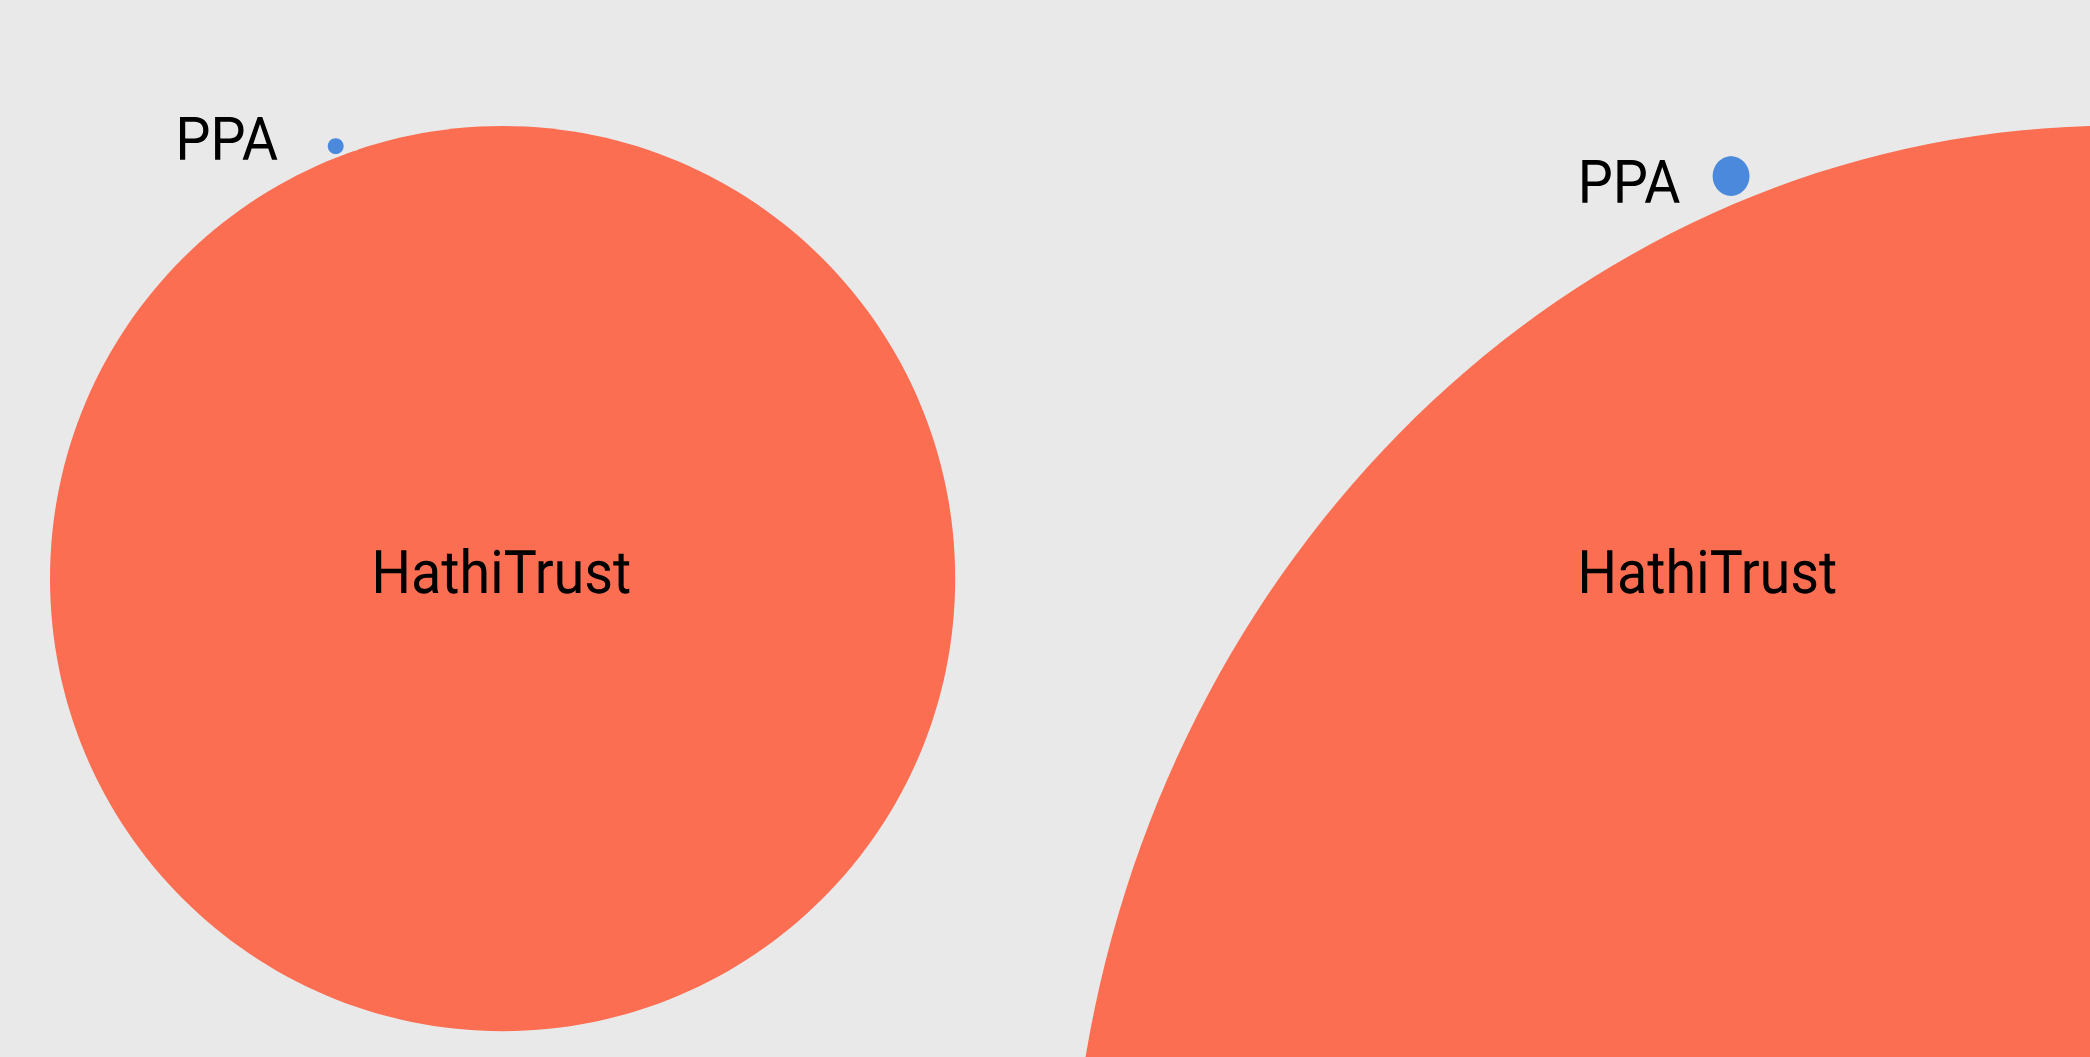
\includegraphics[width=0.75\linewidth]{figures/bubble-chart.png}
    \caption{This bubble chart, originally published in Rebecca Sutton Koeser’s essay “Visualizing the Collections,”\cite{koeser_visualizing_2020} shows the relative scale of HathiTrust and PPA as of 2020. At the time of writing, the PPA contains 5,480 HathiTrust works, or 0.025\% of HathiTrust. }
    \label{fig:bubble-chart}
\end{figure}
This vast difference in scale is actually a reason for the PPA’s creation; such a highly specialized discourse would easily get lost when searching the full scale of HathiTrust’s collection. Other, more standard collaborations with HathiTrust than ours share this same motivation. Many HathiTrust-based projects focused on various methods for, first, finding certain kinds of material within HathiTrust’s massive digital library, and then testing various text and data mining methods on that collection using the tools and services provided by HathiTrust Research Center (HTRC)\cite{noauthor_hathitrust_nodate}. Prominent examples of this two-step process include Gioia Stevens’s \textbf{Early American Cookbooks} project (now a permanent collection within HathiTrust) \cite{stevens_new_2017} and Laure Thompson and David Mimno’s \textbf{20th Century English-Language Speculative Fiction }(a recommended workset within HTRC) \cite{thompson_laure_building_nodate} \cite{noauthor_recommended_nodate}. Recent work from Ryan Dubnicek and various collaborators has focused on using machine learning methods to discover particular genres within HathiTrust Digital Library \cite{parulian_uncovering_2022} \cite{dubnicek_ryan_piloting_2023} and building out the customizable capacities of HTRC’s Extracted Features dataset through the development of an open API \cite{john_a_walsh_library_nodate}. While this work has been important, the algorithms, datasets, and advanced computing environments are all contained within HTRC’s “walled garden,” a closed platform with controlled access and limited interactions. Part of what makes the case of the PPA so unusual is that it brings HathiTrust’s data out of the “walled garden” and puts it in conversation with works that are not found in HathiTrust: eighteenth-century tracts owned by Gale/Cengage, and early modern works from EEBO-TCP. We believe that working across walled gardens is the future of computational scholarship, as evidenced by the sunsetting of JSTOR’s TDM platform Constellate on July 1, 2025 \cite{noauthor_constellate_2019} and HathiTrust’s announcement in October 2024 that it was shutting down the HTRC because “many of our members have rarely utilized HTRC’s services,” leaving the future of TDM on HathiTrust works uncertain \cite{noauthor_plans_nodate}.

Cutting across walled gardens to incorporate works from Gale/Cengage’s ECCO into the PPA introduced different kinds of instability. Indeed, the ECCO data provides an interesting counterpoint to the instability of HathiTrust: the data itself is unchanged, and the OCR text for these materials have not been updated since 2008, even though there have been substantial improvements in OCR technology since the collection was originally digitized, in spite of the known poor quality of the text \cite{hill_quantifying_2019}. In this case, we encountered instability in the technical and human infrastructure. In the time since we first added the integration in 2021, Gale/Cengage made changes to its API that broke our image thumbnails, as well as the PPA links to ECCO for non-Princeton users. These changes required work on our part to adapt our systems and fix the issues. As with HathiTrust, we have also encountered personnel turnover, where our key contacts and collaborators have left without notice. Although our agreements with these institutions are formalized in MOUs, or Memoranda of Understanding, they generally view our project as an exception or experiment for an unusual use case, so there is no plan for continuity when our contacts leave, as we have discussed elsewhere\cite{naydan_beyond_2024}. 

It is difficult to identify other digital projects with unusual uses of data or technical infrastructure from an outside perspective; this requires insider knowledge of the process of working with vendors to build projects, which is less often narrated than research methods, analytical results, or final outputs. Meredith Martin’s new monograph, \textit{Poetry’s Data}, is a notable exception to this trend and argues for the value of narrating the process of navigating our digital research infrastructures \cite{martin_poetrys_2025}. From our experience, the Princeton Geniza Project and the Shakespeare \& Company Project are two additional examples of unexpected uses, since they both use IIIF in unintended ways \cite{noauthor_princeton_nodate} \cite{noauthor_shakespeare_2020}.   

\subsubsection{The problem of excerpts}

The most unusual aspect of PPA’s use of HathiTrust is arguably its support for book excerpts and journal articles. HathiTrust scans and indexes full works and full volumes of journals; it does not provide any consistent, reliable, or systematic semantic structure to identify the chapters or articles contained within them. After our initial launch in 2019, however, it quickly became clear that excerpt-level indexing would surface discoveries that would otherwise remain buried beneath bad metadata [\href{https://prosody.princeton.edu/editorial/2024/08/book-excerpts-journal-articles-and-better-metadata/}{cite}]. Between 2020 and 2021, the PPA project team worked to identify relevant journal articles and book chapters within larger works and curated the excerpt-level metadata manually. 

\section{Quantifying HathiTrust’s rate of change}

\subsection{Details} \label{sec:intro_details}

You may also include subsections if they help organize your text, but they
are not required. Use as many sections and subsections with whatever names work
for your submission!

\paragraph{Another tip.} In some cases, it may be helpful to use \texttt{paragraph} to title individual paragraphs. For example, if a section describes features for a classifier, you can optionally title each paragraph with the name of each feature. 

\section{Elements}

\subsection{Citing elements}

Here are some examples of how to construct and reference common elements in LaTeX. References to elements such as tables, figures, equations and sections make use of \texttt{label} names that you set. References to citations should use the labels you indicate in \texttt{bibliography.bib}. Change all of these examples and values with your own data. 

We can cite Table~\ref{tab:example} as well as Figure~\ref{fig:example}, and we also cite an example paper \cite{tettoni2024discoverability}.
We can also include mathematical notations, such as:
\begin{align}
f(y) &= x^2. \label{fig:squared}
\end{align}
The line number of the equation can be cited as
Equation~\ref{fig:squared}. You can also cite multiple papers together \cite{barré2024latent, levenson2024textual, bambaci2024steps}, and reference figures or tables indirectly in parentheses (Figure~\ref{fig:example_bigger}). You can also cite other sections or subsections of your paper, such as \S\ref{sec:intro_details}. 


\begin{table}[h]
  \centering 
  \begin{tabular}{cc}
    \toprule
    Column Name 1 & Column Name 2\\
    \midrule
    d1 & d2 \\
    d1 & d2 \\
    d1 & d2 \\
    \bottomrule
  \end{tabular}
  \caption{Example table and table caption.}
  \label{tab:example}
\end{table}


\subsection{Required specifications}

Tables and figures should \textit{not} appear at the top of the first page above the paper title and abstract, but can be placed within the main text, as exemplified by Table~\ref{tab:example}. They may also be placed at the top of non-first pages, as exemplified by Figures~\ref{fig:example} and \ref{fig:example_bigger}. Figures and tables discussed in the main text should appear \textit{before} the References section. Supplementary materials should be referenced by their relevant Appendix section, such as Appendix~\ref{appdx:first}. 

Do \textit{not} change the font size of table and figure captions, or the spacing between text lines, section/subsection titles, tables, figures, and captions. You should size your figures and tables so that they stay within the \texttt{linewidth} of the paper. 

\begin{figure}[t!]
  \centering
  
\includegraphics[width=0.4\linewidth]{640x480.png}
  \caption{Example figure and figure caption.}
  \label{fig:example}
\end{figure}

\begin{figure}[t!]
  \centering
  
\includegraphics[width=0.4\linewidth]{640x480.png}
  
\includegraphics[width=0.4\linewidth]{640x480.png}
  \caption{Example figure, where two \texttt{.png} are placed side by side.}
  \label{fig:example_bigger}
\end{figure}


testing figures


\begin{figure}[t!]
  \centering
  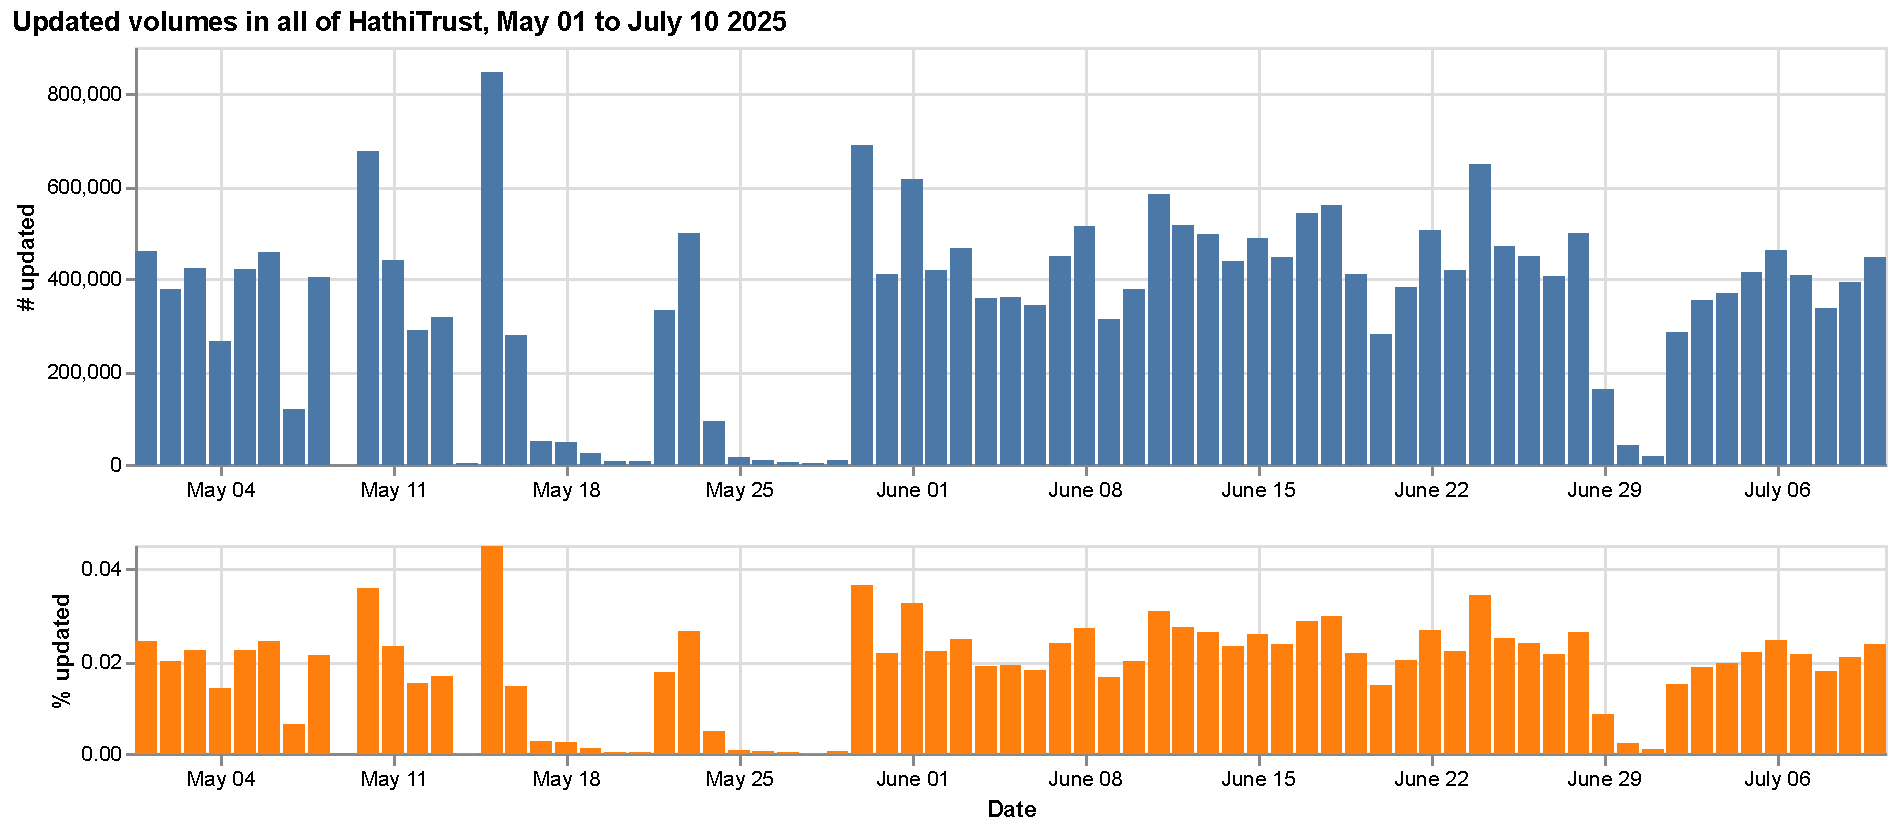
\includegraphics[width=\linewidth]{figures/hathitrust_changes.pdf}
  \caption{changes in HT over time.}
  \label{fig:ht_updates}
\end{figure}


\begin{figure}[t!]
  \centering
  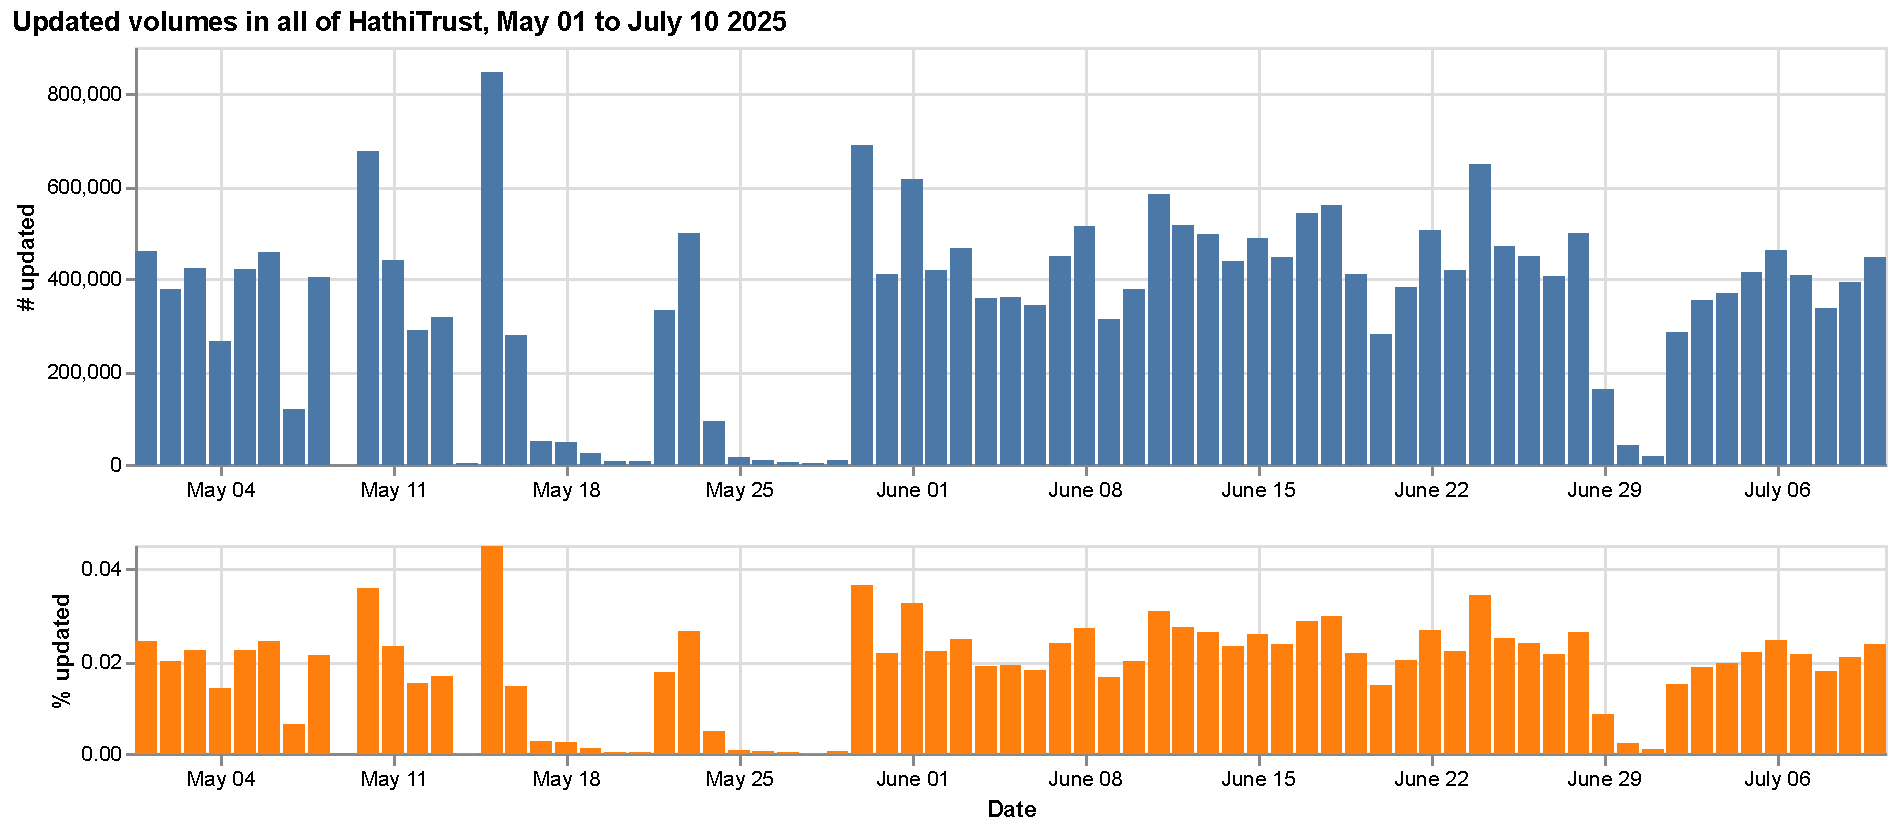
\includegraphics[width=\linewidth]{figures/ppa_hathitrust_changes.pdf}
  \caption{changes in PPA HT volumes over time.}
  \label{fig:ppa_ht_updates}
\end{figure}


\begin{figure}[t!]
  \centering
  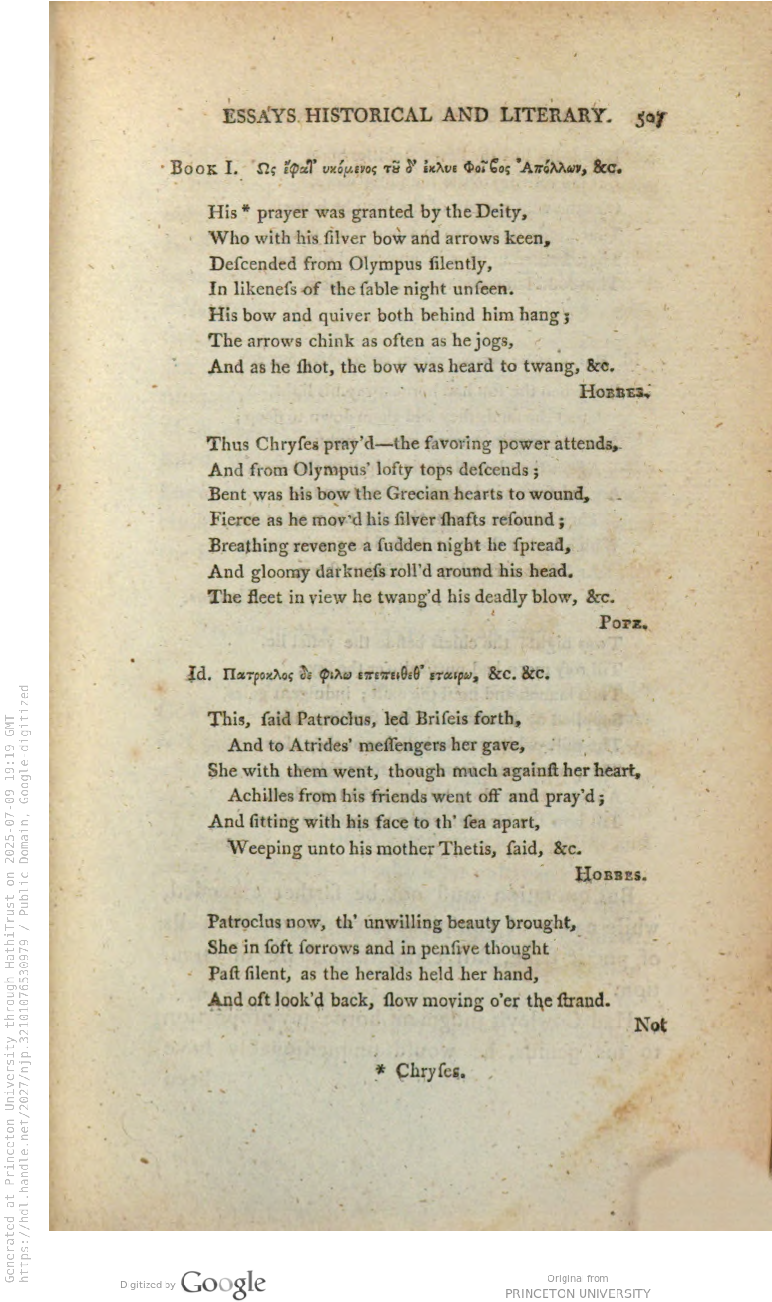
\includegraphics[width=0.4\linewidth]{figures/hathi-pages/njp-32101076530979-515-1752088772.pdf}
  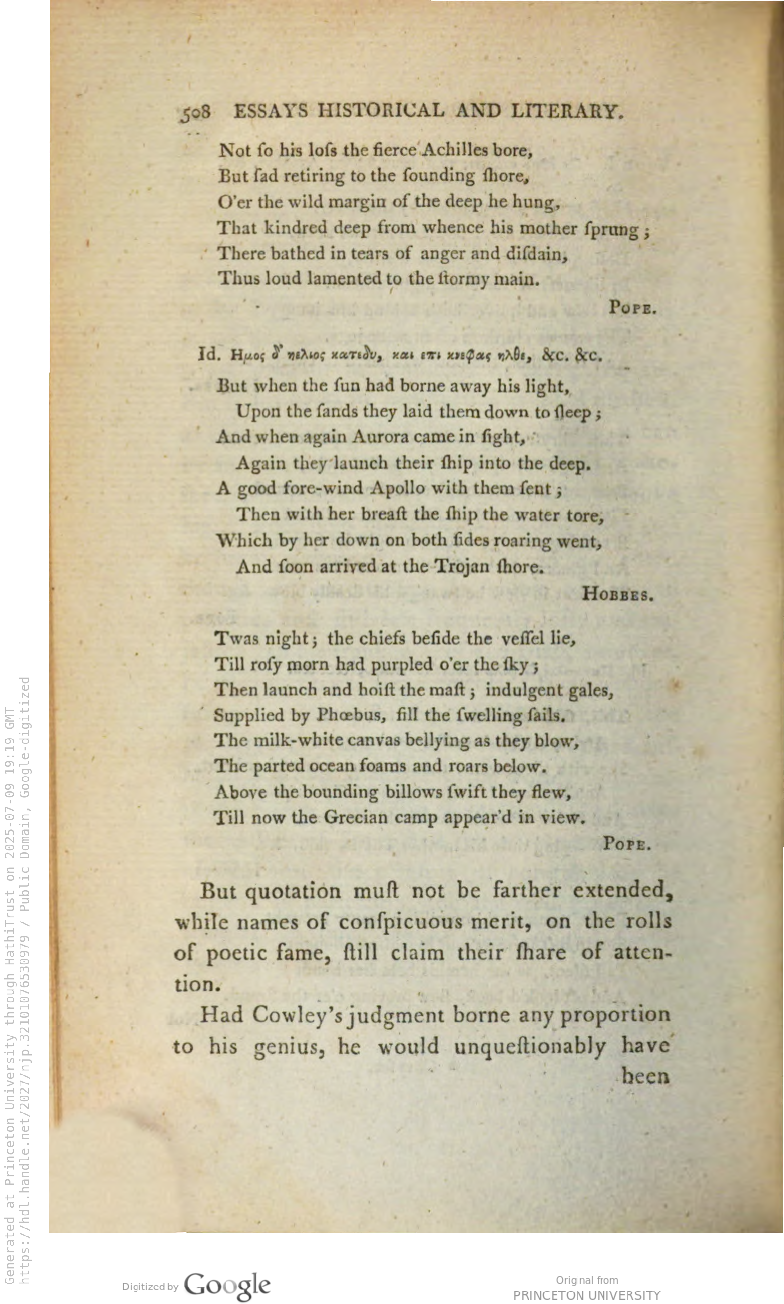
\includegraphics[width=0.4\linewidth]{figures/hathi-pages/njp-32101076530979-516-1752088741.pdf}
  \caption{Two pages all or almost poetry with genre labels of poetry.}
  \label{fig:poetry_pages}
\end{figure}

\begin{figure}[t!]
  \centering
  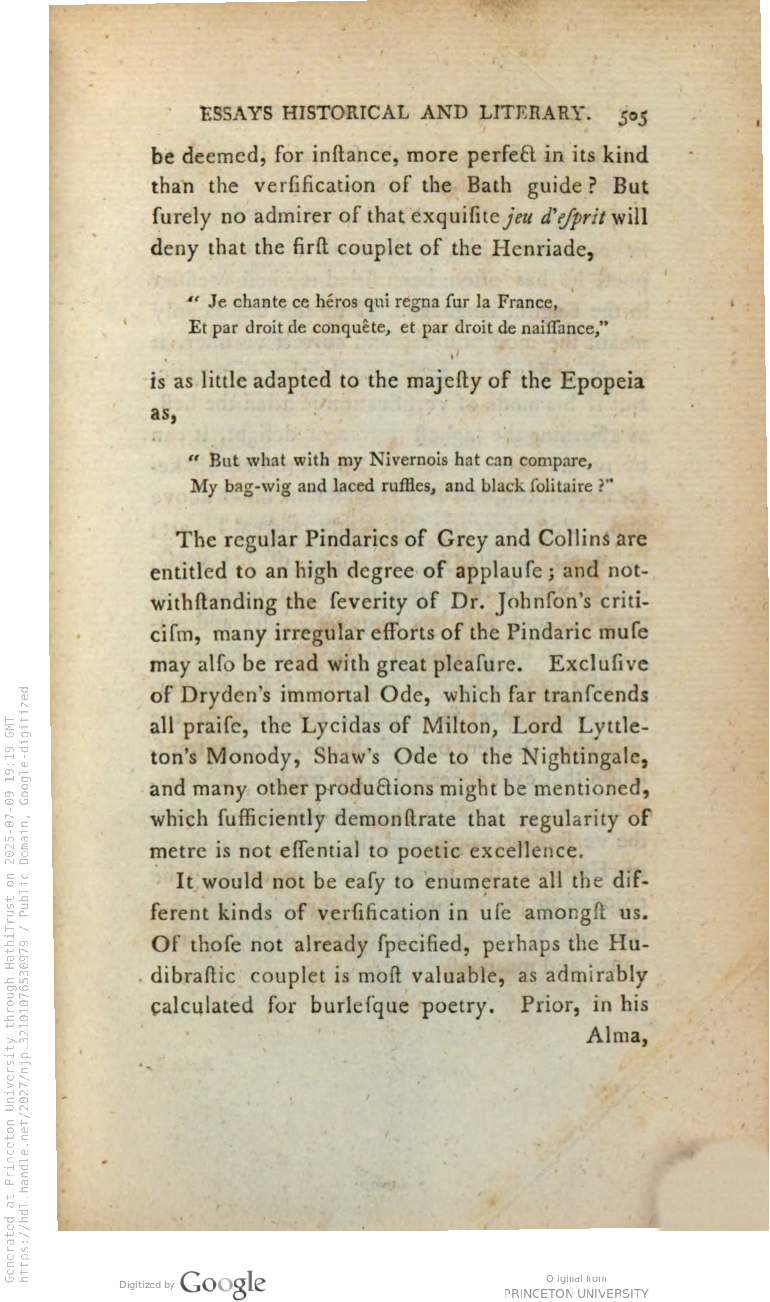
\includegraphics[width=0.4\linewidth]{figures/hathi-pages/njp-32101076530979-513-1752088792.pdf}
  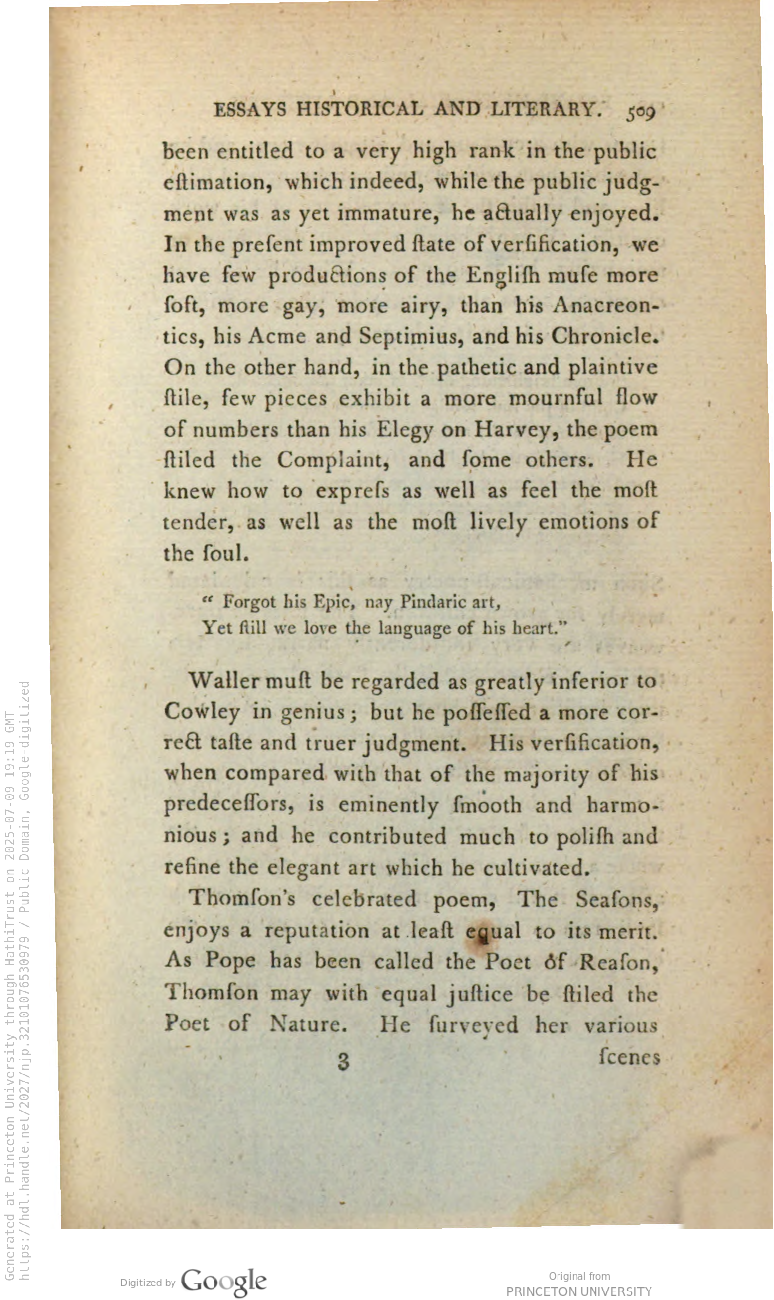
\includegraphics[width=0.4\linewidth]{figures/hathi-pages/njp-32101076530979-517-1752088752.pdf}
  \caption{Two pages with poetry excerpts not labeled as poetry.}
  \label{fig:poetry_exc_pages}
\end{figure}

testing a different option for page images, 4up 

\begin{figure}[t!]
  \centering
  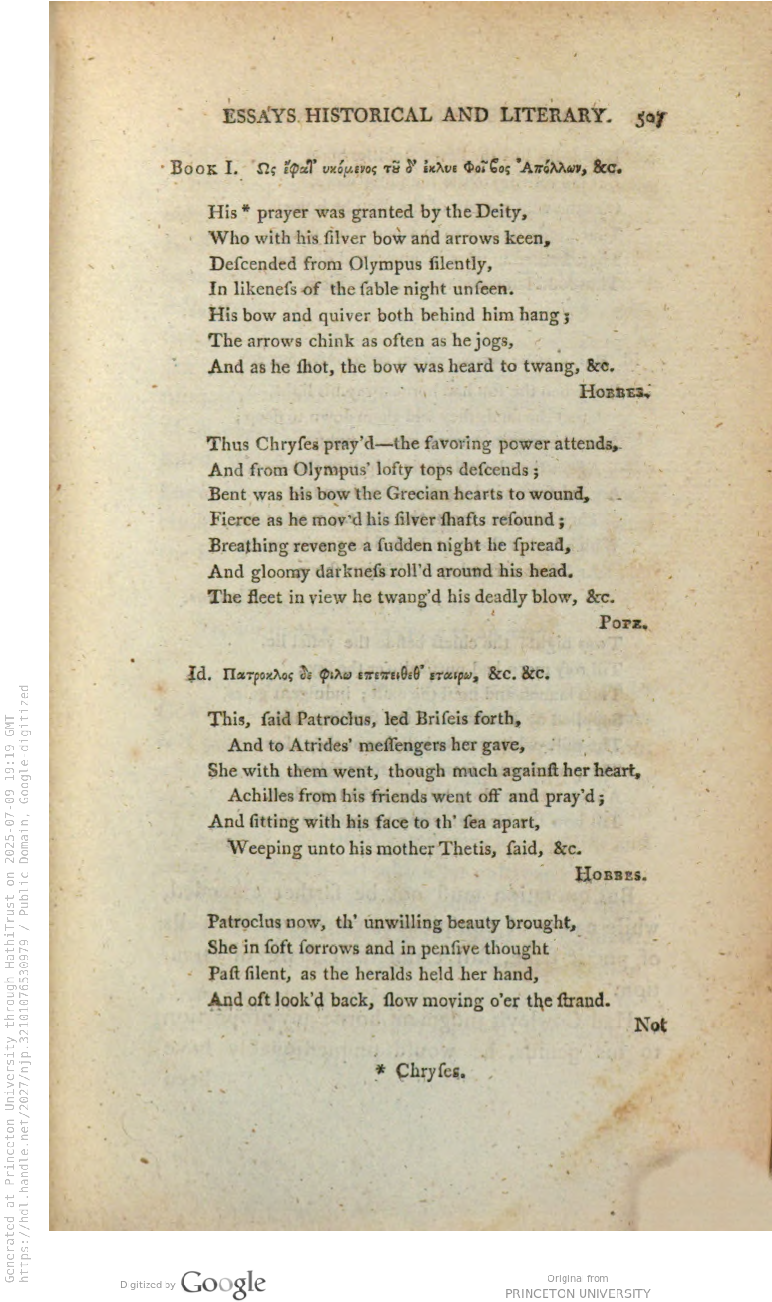
\includegraphics[width=0.24\linewidth]{figures/hathi-pages/njp-32101076530979-515-1752088772.pdf}
  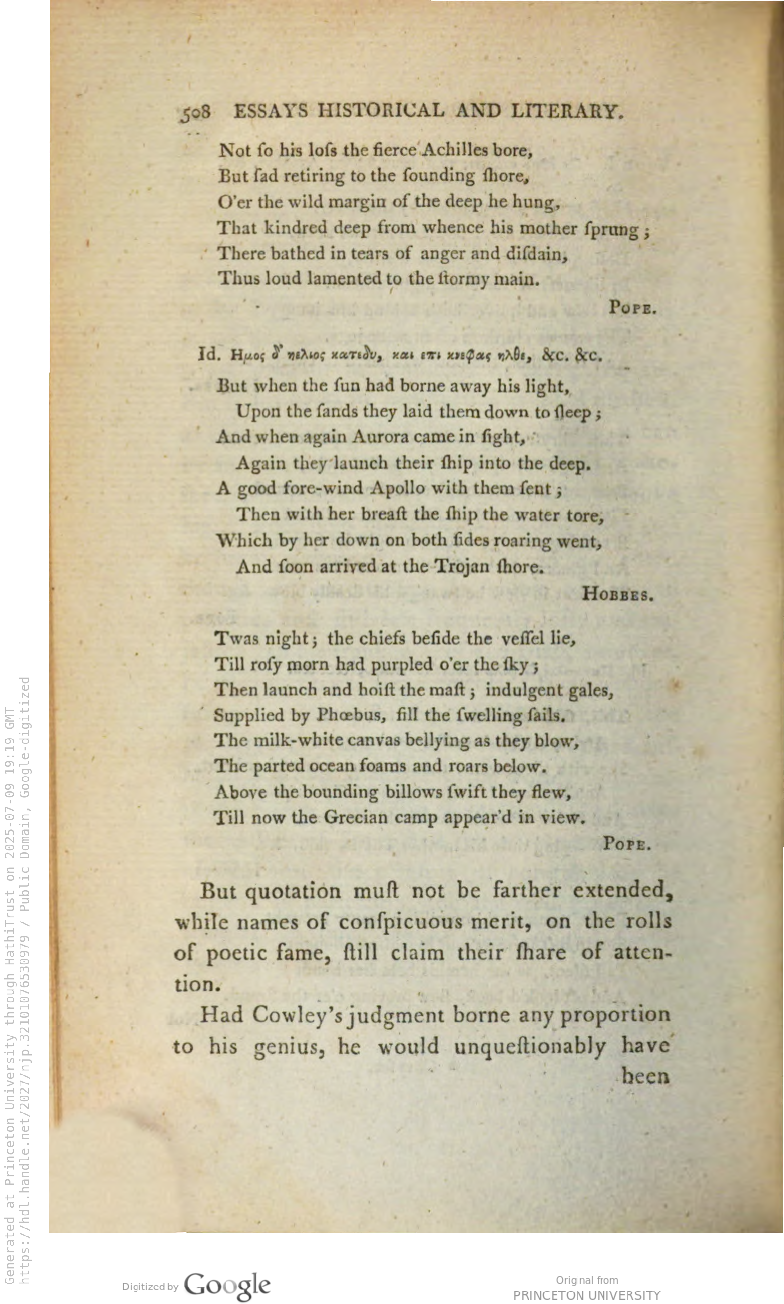
\includegraphics[width=0.24\linewidth]{figures/hathi-pages/njp-32101076530979-516-1752088741.pdf}
  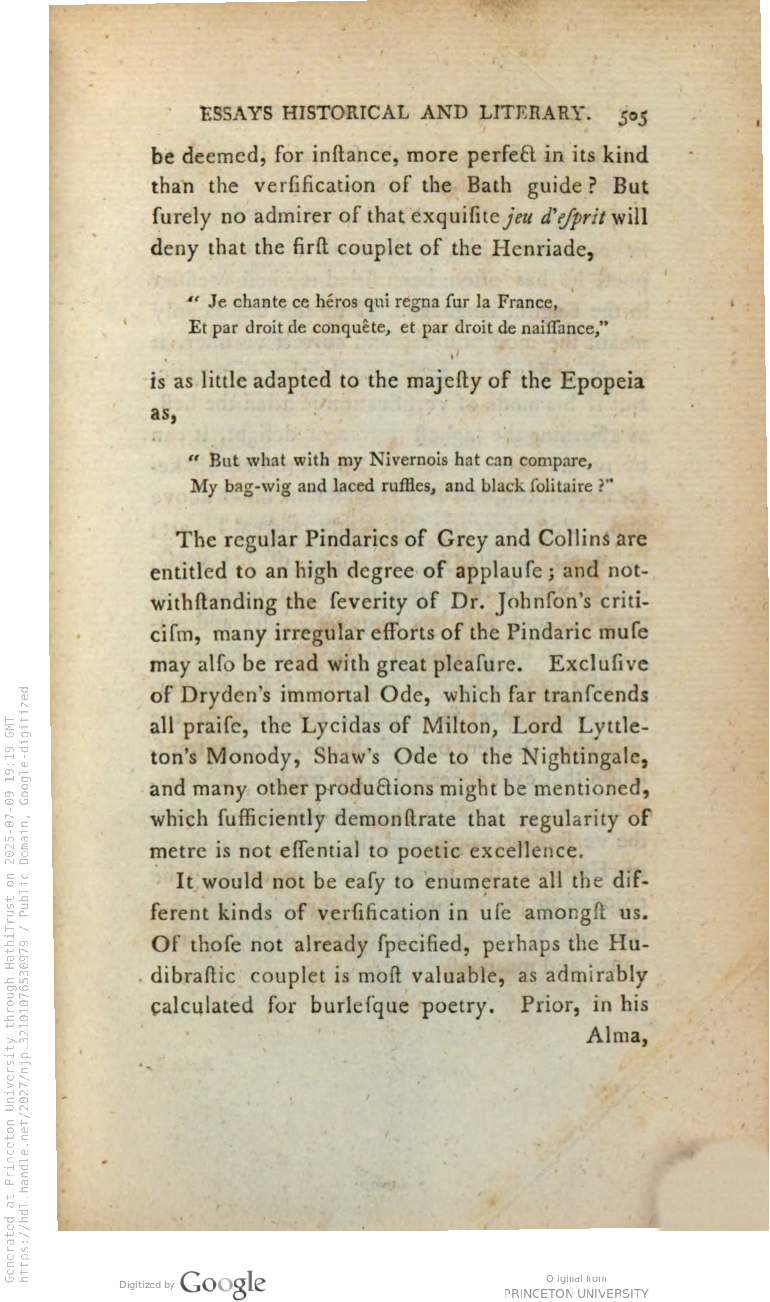
\includegraphics[width=0.24\linewidth]{figures/hathi-pages/njp-32101076530979-513-1752088792.pdf}
  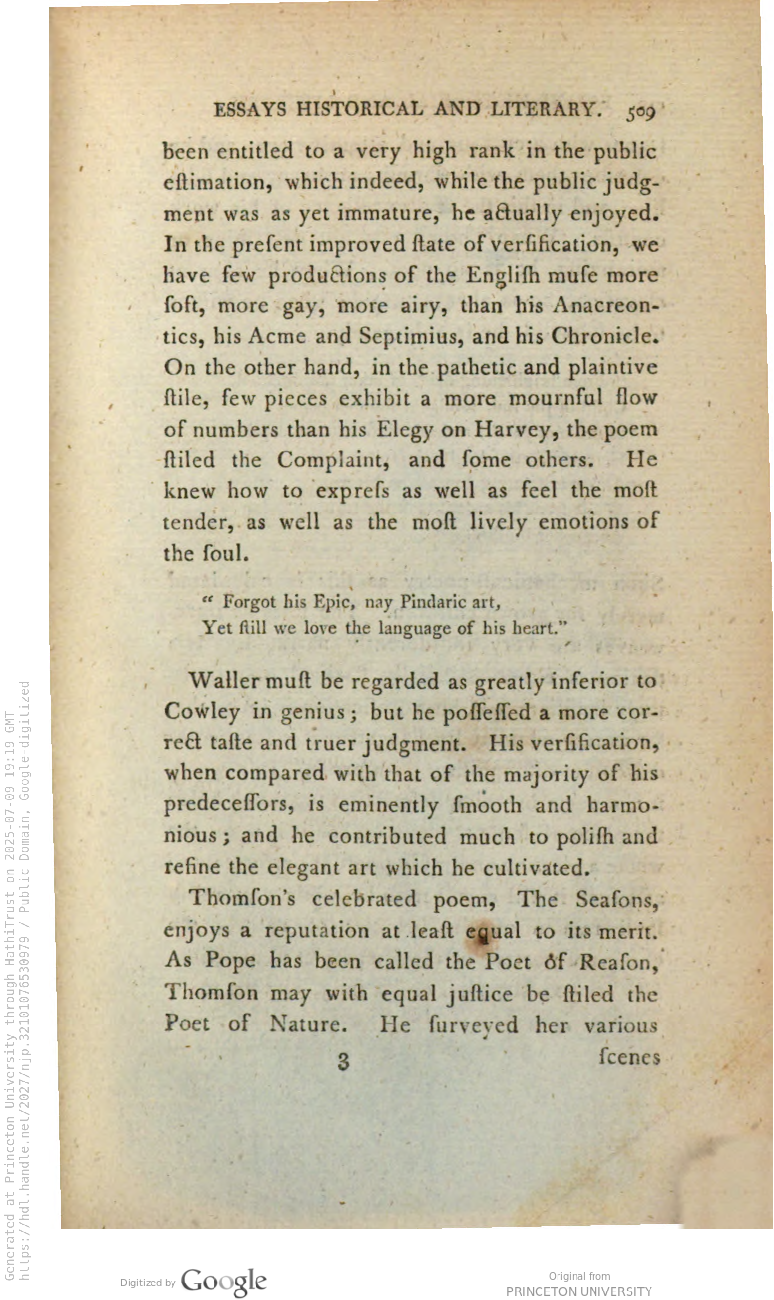
\includegraphics[width=0.24\linewidth]{figures/hathi-pages/njp-32101076530979-517-1752088752.pdf}
  \caption{Pages with poetry and poetry excerpts.}
  \label{fig:poetry_pages}
\end{figure}



\section*{Acknowledgements}

This unnumbered section should be blank when submitting your paper. After review, you may include lists of people and organizations who supported the work.

% Print the biblography at the end. Keep this line after the main text of your paper, and before an appendix. 
\printbibliography

% You can include an appendix using the following command
\appendix

\section{HathiTrust Statement for Dataset Distribution} \label{appdx:first}

By my signature, I acknowledge and confirm the following:

\begin{enumerate}
    \item  I am receiving texts from the University of Michigan that are made available under an agreement between my sponsoring institution - [indicate sponsoring institution, e.g., Dartmouth College] - and Google.
    \item  I have read this agreement and agree to abide by its terms and to use the texts in accordance with the statement of my research, as submitted to the University of Michigan.
    \item  I agree to notify the University of Michigan of any changes that are made in the scope or nature of my research.
    \item  I understand that volumes I receive from the University of Michigan may be determined at a later date to be in copyright. I agree to delete these volumes and any copies that have been made upon notification from the University of Michigan. I agree to notify the University of Michigan at feedback@issues.hathitrust.org to confirm deletion of any such volumes.
\end{enumerate}

\rule{\textwidth}{0.5pt}

Name \hspace{0.3\textwidth} Signature \hspace{0.3\textwidth} Date

\rule{\textwidth}{0.5pt}

Title

\rule{\textwidth}{0.5pt}

Email \hspace{0.3\textwidth}  Phone


\section{Example HathiTrust deletion email for public domain dataset} \label{appdx:second}

\begin{verbatim}
Subject: Delete notifications for ht_text_pd dataset
From: HathiTrust <support@hathitrust.org>

Dear HathiTrust dataset recipient,

This email is to notify you that volumes in the HathiTrust
"ht_text_pd" dataset, of which you have downloaded all
or a subset of files, no longer meet the criteria for
inclusion in the dataset, and you no longer are allowed to
use them in your research.

Please review the data you have synced from HathiTrust to
check whether you have the volumes listed below. If so,
delete all copies you retain of these volumes in
accordance with our terms of use. Alternatively, you may
delete your copy of the dataset and re-sync to the updated
dataset.

If you no longer possess HathiTrust datasets, or if you
have other questions regarding datasets, then please email
support@hathitrust.org.

Thank you,

HathiTrust

===BEGIN ID LIST===
[ids omitted]
...
...
...
===END ID LIST===

\end{verbatim}
\end{document}
